\documentclass[a4paper,11pt]{article}
\usepackage[latin1]{inputenc}
\usepackage{times}
\usepackage[T1]{fontenc}
\usepackage[english]{babel}
\usepackage{latexsym}
\usepackage{tipa}
\usepackage{pictex}
\usepackage[authoryear,round]{natbib}
\setcounter{secnumdepth}{0} \linespread{1.5}
 
\usepackage{amsmath}
\usepackage{amssymb}
\usepackage[usenames,dvipsnames]{color}
\usepackage{graphicx}
\usepackage{verbatim}
\usepackage{amsmath}
\usepackage{amsfonts}
\usepackage{amssymb}
\usepackage{latexsym}
\usepackage{natbib}
\usepackage{xr}
\usepackage{setspace}
\usepackage{framed}
\usepackage{cancel}

\newcommand{\comb}[2]{{#1 \choose #2}}
\newcommand{\mosr}[1]{{ #1}}

\newcommand{\beginsupplement}{%
        \setcounter{table}{0}
        \renewcommand{\thetable}{S\arabic{table}}%
        \setcounter{figure}{0}
        \renewcommand{\thefigure}{S\arabic{figure}}%
}

\begin{document}

\title{Association of adaptive phenotypic traits to causal variants using the extended genotype homozygosity matrix.}
%\author{Sebastian E. Ramos-Onsins, Ioanna Theoni Vourlakis, \\ Josep Ma. Folch, Armando Caballero, Miguel P\'erez-Enciso\\ (Contributed: not yet the real order)}
\date{\today}
\maketitle

\section{Abstract}

TO DO ...

\section{Introduction}

The detection of the effect of adaptive phenotypic traits is fundamental for understanding the number of affected variants and the strength of selection for these adaptive traits. The detection of the association between an adaptive phenotype and the genotype can be difficult, depending on the effect of each associated variant and the effect of the adaptation over the positions around it. A number of studies, which the aim of understanding the patterns of frequencies for adaptive traits  \citep[\textit{e.g.},][]{Eyre-Walker:2010aa,Caballero:2015aa,Lourenco:2011aa,Connallon:2015aa}, shown that the genome architecture for a trait depends on the (mathematical) relationship of the trait versus fitness (that is, if the fitness is directly correlated with the trait or, alternatively, fitness and traits are correlated distributions). Simons et al. (2018) avoided this problem by inferring the relationship between trait and fitness from empirical data and estimated the genetic architecture of the trait, assuming pleiotropy and stabilizing selection. Also, \citet{Beissinger:2018aa} developed a test to detect the effect of selection on a quantitative complex trait using the whole information on effect sizes.\citet{Uricchio:2019aa}  developed a new method to detect the signals of polygenic selection using the derived allele effect size from GWAS analysis and the derived allele frequency of the associated variants. All of these methods can be applied to observe the effects of environmental changes on the genome for specific traits related to adaptation. Recently \citet{Zeng752527} developed a bayesian algorithm (SBayesS) that requires GWAS summary statistics and functional genomic annotation to detect the effect of selection on complex polygenic traits. 

Here, we are aimed to (i) discover if a given trait is under a recent adaptive process and (ii) to detect strong and medium adaptive effects with higher precision, based on the association of the trait versus phenotype. We propose to use the signals of linkage disequilibrium produced by causal adaptive variants to increase the precision in locating associate variants as well as distinguishing  between adaptive versus non-adaptive variants. The reasoning is the following: the causal variants of an adaptive trait will left signals of adaptation (\textit{e.g.,}, increase of homozygosity around the causal variants, more linkage disequilibrium, reduction of variation) around them. If a trait is under adaptive pattern, we expect that the associated variants exhibit signals of adaptation, while other non-adaptive traits will not have such signals on associated variants. Additionally, the signals of adaptation may increase the precision to locate the causal variants, together with the genotype data. 

We propose to study the association between the phenotype and the genotype considering  additionally (as additional genotype information)  a matrix containing the extended genotype homozygosity.  This matrix would be used in the analysis of association to detect the effect of adaptive selection of the studied phenotype. %If we consider a single population that have suffered a strong selective event, those causal positions that strongly determined the selective effect will increase rapidly their frequency, and thus will have larger linkage disequilibrium with the closest sequences than other regions not affected by selective events.  With this idea it is pretended to take advantage of the stronger footprint of a sweep associated to a selective event  to give more weight to those individuals in whose the studied position contains a determinant allele, as well as longer linkage in close regions caused by the effect of the selective sweep. 
Our hypothesis is that this approach can have  promising results to detect the causal mutations in panmictic populations that have experimented stronger selective events. %On the other hand, this approach should not not give additional information in association studies designed to distinguish between divergent admixed populations (and neither control-disease populations). 
A consistent simulation study is required in this project to evaluate different scenarios.

%The GWAS analysis with a single panmictic population is based on the association analysis of a single variant position for each of the individuals (usually genotype information, that is, a variable with  the discrete values 0, 1 and 2, indicating the number of copies of a variant - reference or alternative -), considering the relationship between individuals and other variables, versus the observed phenotype at each of the individuals. Thus, it is crucial to define all the genetic features at the studied position for each individual. One of this genetic features is the degree of homozygosity/heterozygosity in neighbouring regions to this position at each of the individuals. The presence of causal variants close to a given position and the observation of homogeneity of the individual at this region will, presumably, be associated with the phenotype. The larger homogeneity on the focus position with their neighbouring region may indicate a causal effect.

The resolution of this kind of statistics is expected to be in the range of genetic breeding improvement up to domestication process (approximately from some dozens to hundreds of generations (less than $N_e$ generations, \citep{Sabeti:2002aa}. This range may allow to detect critical traits and the effect of these traits on the genome under crucial events such as the domestication. In this work, the statistics used are calculated at genome level %for unphased data
, which are analyzed with the phenotypes of individuals.

\section{Methods}
\subsection{Considering a single population and polarized alleles (ancestral and derived)}
Following \citet{Sabeti:2002aa}, we define the statistic $EHH_d$ as the proportion of homozygote individuals of the derived allele from position $i$ (the target position) to position $j$, in relation to the number of homozygote individuals with derived variants at the position $i$ (note that derived variants are obtained by comparison to an/several outgroup species).  That is:

 \begin{equation}
 EHH_{d_{ij}} = \frac{\sum_{k=1}^{n}I_{d_{k,ij}}}{\sum_{l_d=1}^{n}I_{d_{l,i}}},
 \end{equation}
where $n$ is the number of individual samples, and $I_{d_{k,ij}}$ counts 1 if the individual $k$ is homozygote for derived variant at position $i$ and is still homozygote from position $i$ to $j$, otherwise counts 0. In the same way, $I_{d_{l,i}}$ counts 1 if the individual $l$ is homozygote for derived at position $i$, otherwise counts 0. The statistic $EHH_a$ is calculated in the same way than $EHH_d$ but considering ancestral variant instead of derived variant.  %
Note that this value can not be calculated in case there are not derived (ancestral) homozygous individuals.
%In case there are no derived homozygotes at position $i$, we define $EHH_{d_{ij}} = 0$. Same for ancestral.

In order to quantify the effect of the neighbouring homozygosity at a given studied position ($i$),  all values for $EHH_{ij}$ are summed from the position $i$ to their right and and to their left sides considering their distance (physical or recombinant), and until reaching a threshold arbitrary value of $EHH_{ij}$ (let's say 0.1). That is: 

\begin{equation}
 iES_{d_i} = \sum_{j=x+1}^{y}\frac{(EHH_{d_{ij-1}} + EHH_{d_{ij})}}{2} (Pos_{j} - Pos_{j-1}),
 \end{equation}
 $x$ and $y$ are the positions (at the right and at the left) where $EHH_{d_{ij}}$ becomes below the threshold or it is too far (by the presence of large gaps) from the central position (so the area out of $x$ and $y$ is considered unimportant), and $Pos$ is the physical or the recombinant position (from a linkage map). The same is for the ancestral statistic ($iES_{a_i}$).

The integrated relative Extended homozygosity statistic is then calculated as:
 \begin{equation}
 iRES_{da_{i}} = \frac{iES_{d_{i}}} {iES_{a_{i}}}.
 \end{equation}
A value higher than 1 (if the genotype extension statistic for derived variants is larger than for ancestral variants) suggest the effect of positive selection favouring a derived variant at position $i$.  

\subsubsection{The homozigosity at each position per individual}
In case of doing a GWAS analysis, usually each position and genotype is evaluated independently in relation to each individual phenotype. That means that it is crucial to distinguish the genetic information between individuals at this position. Here we propose to include the information concerning to the homogeneity of the individual at neighbouring regions from the focus position (that is, a way to consider the linkage disequilibrium between the two chromosome copies of an individual at this region) in addition to the genotype at the focus position. That is, it is calculated a statistic related to the neighbouring homogeneity for every position and individual. This statistic is obtained by slicing the $iRES_{da_i}$ statistic given the contribution of each individual ($k$) to the total:

\begin{equation}
\begin{split}
%\begin{align}
iES_{dk_i} = \sum_{j=x+1}^{y}(EHH_{d_{k,ij-1}}+ EHH_{d_{k,ij}})(Pos_{j} - Pos_{j-1}) / 2, \text{ and }\\ 
iRES_{da_{k,i}} =  \frac{iES_{d,k_i}}{iES_{a}},
%\end{align}
\end{split}
\end{equation}
where $x$ and $y$ are the positions (at the right and at the left boundaries for derived) and $EHH_{d_{k,ij}} = I_{d_{k,ij}} / (\sum_{l_d=1}^{n}I_{d_{l,i}})$. 

\subsection{Quantifying homogeneity with no outgroup and unphased data}
To quantify the homogeneity with no outgroup and unphased data, it is convenient to use the framework developed by \cite{Tang:2007aa} to study the degree of homogenization of a given position (using unphased genotype information) as is explained below.

\subsubsection{Define candidate positions}
 In a first step, it is useful to define those candidate positions in relation to their maximum local extension of their homozygosity. This step is optional, as other criteria for defining candidate positions can be used. Following \citep{Tang:2007aa}, we define $EHHS_{ij}$ as the proportion of homozygote individuals from position $i$ (the position of interest) to position $j$, in relation to the number of homozygote individuals at the position $i$. That is:
 
 \begin{equation}
 EHHS_{ij} = \frac{\sum_{k=1}^{n}I_{k,ij}}{\sum_{l=1}^{n}I_{l,i}},
 \end{equation}
where $n$ is the number of individual samples, and $I_{k,ij}$ counts 1 if the individual $k$ is homozygote from position $i$ to $j$ (\textit{i.e.}, using the genotype nomenclature, all variants have the values 0 or 2 at this region), otherwise counts 0. In the same way, $I_{l,i}$ counts 1 if the individual $l$ is homozygote at position $i$, otherwise counts 0. This statistic is calculated from position i to any position (left or right) until this proportion becomes enough small to be considered negligible. This threshold value, although is somewhat arbitrary, it has been considered 0.1 in the original work \citep{Tang:2007aa} and here it is used the same criteria. The $EHHS_{ij}$ values for the position $i$ are kept and used to calculate the next statistic $iES_i$ \citep{Tang:2007aa}.

The following calculation of the $iES_i$ statistic pretends to quantify the effect of the neighbouring homozygosity at a given studied position. Having all values for $EHHS_{ij}$, we count the total area of homozigosity around the position $i$, that is, having the position $i$ as the center, we sum, at their right and and their left, all the contributions of $EHHS_{ij}$, considering their distance (physical or recombinant). that is: 

 \begin{equation}
 iES_i = \sum_{j=x+1}^{y}\frac{(EHHS_{ij-1} + EHHS_{ij})}{2} (Pos_{j} - Pos_{j-1}),
 \end{equation}
where $x$ and $y$ are the positions (at the right and at the left) where $EHHS_{ij}$ becomes bellow the threshold or it is too far (by the presence of large gaps) from the central position (so the area out of $x$ and $y$ is considered unimportant), where $Pos$ may be the physical or the recombinant position (from a linkage map).
 
\subsubsection{The homogeneity at each position per individual using unphased and no outgroup data}
As explained above, for GWAS analyses it is convenient to have information of the homogeneity per individual (to be contrasted with phenotype data). The desired  statistic is obtained by dividing the $iES_i$ statistic given the contribution of each individual to the total:

 \begin{equation}
 iES_{k,i} = \frac{1}{2\sum_{l=1}^{n}I_{l,i}} \sum_{j=a+1}^{b} (Pos_{j} - Pos_{j-1}) (I_{k,ij-1} + I_{k,ij}),
 \end{equation}
where $\sum_{k=1}^{k=n}iES_{k,i}=iES_i$ (considering the same threshold values -$a$ and $b$- for the each of the samples, lke $iES_i$ statistic). Here the only differential term between individuals (in relative terms) is the last sum. % Note also that the term $2\sum_{l=1}^{n}I_{l,i}$ can be eliminated from the equation because %
%That is, the objective here is the difference between individuals and not the absolute value. Therefore:

%Additionally, if we want to count not only the homogeneity in homozygous positions but also in heterozygous positions, we can define $I'_{k,ij}$, where it counts 1 if the genotype between $i$ and $j$ are completely homozygous or completely heterozygous.  %
%Then the new statistic $iES'_{k,i}$ will consider also heterozygous regions (for example, in case having advantage for heterozygotes). That is:

%\begin{equation}
% iES'_{k,i} = %
%%% \frac{1}{2\sum_{r=1}^{n}I_{r}} \sum_{j=a+1}^{b} (Pos_{j} - Pos_{j-1}) (I'_{k,ij-1} + I'_{k,ij}) \propto 
%%{\sum_{j=a+1}^{b} (Pos_{j} - Pos_{j-1}) (I'_{k,ij-1} + I'_{k,ij})}.
%(\frac{1}{2\sum_{l=1}^{n}I_{l,i}} \sum_{j=a+1}^{b} (Pos_{j} - Pos_{j-1}) (I_{k,ij-1} + I_{k,ij}))/iES_i,
%\end{equation}
%and $\sum_{k=1}^{k=n}iES'_{k,i}=1$.
%%The limit of the positions ($a$ and $b$) can be set to those positions where the sum of all $I'_{k,ij}$ in relation to the number of individuals drops below 0.1, as the threshold established for the statistic $iES_i$. 

\subsubsection{Using a reference population: The quotient between the extension of homozygosity in target individuals from a population versus a reference population}
Following the same reasoning, it is possible to estimate the effect of the extension of homozygosity per position and per individual in relation to the effect in a reference population (note that a reference population is not an outgroup species). This is useful in case we are considering the effect of selection in the target population while we assume no selection in the reference population. Those position that have high $iES_i$ at both populations would be considered nuisance given by other factors, like genomic effect caused by the genetic architecture of the genome. Therefore, following \citep{Tang:2007aa}, we define the statistic derived from $Rsb_i$:

\begin{equation}
Rsb_{k,i} = \frac{iES_{k,i}}{iES_{i}^{popRef}}
\end{equation}
where $\sum_{k=0}^{k=n}Rsb_{k,i} = Rsb_i.$

\subsection{The study of association phenotype-genotype and the information related to the homogeneity of individuals in neighbouring regions}
%To perform a study of association genotype-phenotype, we can include the information provided by the statistic $iES_{k,i}$ and $Rsb_{k,i}$ in two different ways: (a) by adding the matrix $iES$ (or $Rsbi$) in replacement of the genotype matrix or (b) using this matrix as a ponderation of the genotype matrix. The two approaches have different meanings and thus different interpretations. In the first case, it is assumed that the homogeneity along the contiguous regions of a position  in a given individual has the same importance than the genotype of this individual, which suggest that regions close to the causal position (not necessarily causal) would be associated. In the second case, the method would stress only those genotypes with an associated phenotype that additionally would have strong ponderation (large homogeneity in the surrounding region). 

%A mixed model is used to associate the phenotype of each individual (a vector $y$ of phenotypes) with the genetic features of the individual at each position (that is, a vector $g$ containing the relation with each individual genotype and a vector $h$ containing the relation with each individual extension of homozygosity versus surrounding positions). For the whole SNPs we relate the phenotype using this general expression:

%\begin{equation}
%y = Wa + Xg + Zh + e ,
%\end{equation}
%where $W$ is a matrix that considers the fixed effects for each individual (related in the $b$ vector), $X$ is a matrix that contains the genotypes of all SNPs and individuals and .$Z$ is a matrix having the extension of homozygosity for each SNP and individual (\textit{i.e.,}, the statistics $iES_{k,i}$ and $Rsb_{k,i}$). Finally, $e$ is the residual error vector. 

A  multivariate regression model has been used to detect the association of a position with the phenotype, considering only, the genotype information, only the extended genotype homozygosity information or both. The probability of association is calculated with the linear model function in R (lm), considering the vector of phenotypes (Y), obtained by summing up (additive model) all the effects per variant position, considering their dominance parameter, in relation to the genotype matrix and/or the ${iES_k}$ matrix  (with a dimension of SNPs x individuals). All these vectors and matrix were normalised previously. The $r^2$ regression value was obtained for each SNP, and the p-value was estimated assuming a $F$ distribution. False discovery rate and Bonferroni methods \citep{Benjamini:1995aa} that correct for multiple testing were applied to raw P-values. \par
To evaluate the capacity that we have to detect real beneficial mutations affecting the studied phenotype we measured the specificity (True Negative Rate) and sensitivity (True Positive Rate or statistical power) for the used matrices (the $iES_k$, the genotype counts and both together). %We are interested in having the maximum specificity as a preference, but also trying to have the maximum statistical power as possible.

%Comparison of the results obtained using GWAS analysis with the extended genotype homozygosity matrix are contrasted  with the test developed by \citet{Beissinger:2018aa}. which identifies selection on complex traits. \par

%DEFINE ASSUMPTIONS, DISTRIBUTIONS  AND SCENARIOS.
\subsection{Simulations}
Forward simulations of a population have been performed with Slim v4  \citep{Haller:2019aa}. A population with 5000 diploid individuals is simulated with a mutation rate of 6e-8 and a recombination rate of 1e-7. A fragment of one million positions is simulated. Mutations type "m2" can be located  in segments of 1Kb in regions separated 100Kb positions. After 40K generations, the population split in two populations with same indiviuals (i.e., $N_e=5000$) and no migration between them.  All mutations start to be neutral, but m2 type mutations start to have an additive effect over the fitness after 50,000 generations. Additionally, once simulations are finished, a non-adaptive  phenotype is constructed from additive effects of random mutations across the genome. This additive effect can be dependent of frequency, such as effect depending on (i) low heterozygosity, on (ii) high heterozygosity and also on (iii) high number of low frequency variants within the population). The model  considers heritability effect on phenotype of h2=0.75 on both adaptive and non-adaptive phenotypes. Populations are evolved until the optimal phenotype value in the population is achieved (an arbitrary small standard deviation of 0.1 close to the optimal) or until arriving 60K generations.

Once simulations are finished, sequences with all variants (in ms format posteriorly translated to genotypes) and phenotypes (in a tabulated format) were kept into files to run Rsbki code, which includes the statistics here developed. The statistics per individual (i.e., iESk, iRESk, Rsbk per individual and position) and the genotype data were used to perform GWA analysis versus individual phenotypes. We expect to identify (some) QTL regions (that is, not all QTLs contain mutations in enough frequency and/or with enough effect to be identified) using standard GWA analysis with genotype data for phenotypes under adaptive effect but also with non-adaptive effect. Nevertheless, it is expected that in case using EHH statistics, only QTLs with phenotypes under adaptation would be identified. This is because the differential signal would only be observed  in positions with adaptation signals. 

%Forward simulations of a population have been performed with Slim v,3 \citep{Haller:2019aa}. A population of 1000 individuals ($N_e$) is simulated. Consider 10 chromosomes of 1Mb (a total of 10Mb), each chromosome including 1000 coding regions of 1.5Kb evenly distributed every 8.5 Kb. We consider mutation rate constant of 1.25e-7 per position and generation, and recombination rate variable following a curve with a minimum peak on the centre of chromosome (rate of 2.5e-8) and increasing logarithmically to achieve a maximum at telomeres (2.5e-5).

%Forward simulations of a population have been performed with Slim v3 \citep{Haller:2019aa}. A population of 1000 diploid individuals ($N_e$) is simulated. We consider 10 chromosomes of 1Mb each (a total of 10Mb), where five chromosomes have no causal variants while each of the remained five chromosomes include 1000 coding regions of 1500bp evenly distributed across the total length. We consider mutation rate constant of 1.25e-7 per position and generation, and recombination rate variable following a curve with a minimum peak on the centre of chromosome (rate of 2.5e-7) and increasing logarithmically to achieve a maximum at telomeres (2.5e-5). The population is run for 10$N_e$ generations and the entire populations is analyzed. Afterwards, a new environment is simulated in this population, and it is continued during 30 more generations. Then, again this new populations is also analyzed.
%
%Functional positions (non-synonymous, defined as the two first positions of each codon) are under selective effects, while non-functional positions are considered neutral. Here, we model positive selection, as we are interested in detecting adaptive events. The new mutations falling in functional positions are under the effect of positive and negative selection: a proportion of mutants will be under positive selection (this ones following an exponential distribution), while the rest will be under negative selection (gamma distribution), according to \citep{Boyko:2008aa} results for human species. 
%
%We have looked at the differences in the distribution of selective and phenotype effects considering the Eyre-Walker proposal \citep{Eyre-Walker:2010aa}, here named EW, and a gamma bivariant distribution \citep{Caballero:2015aa} for negative values (using \textit{simstudy} library in R). The EW distribution estimates the phenotype value from an exponential-like pattern and considering a nuisance parameter, while bivariant gamma distribution is more flexible in considering different patterns of phenotype effects. If we consider an exponential distribution for phenotype effects (shape=1), the distributions are quite similar (see Figure~\ref{comEWvsBiv}). The major difference is observed when comparing distributions with correlation 0, where the observed plot of the EW function is more spread. We decided to use the first option (EW model) because it is possible to estimate easily,  by inversion, the selective effects for an environmental change.
%
%Different scenarios of the relationship between the fitness effect and the phenotypic trait are considered, from no-correlated to highly correlated relationship, using the Eyre-Walker (EW) model \citep{Eyre-Walker:2010aa}, that is, the effect for a phenotype trait $z$ is related to selective effects, $4Ns$, using the equation $z=\delta (4N_e s)^\tau (1+\epsilon)$, where $\delta$ is a given random value (\textit{e.g.},-1 or 1), $\tau$ is related to the correlation of phenotypic trait with the $s$ and $\epsilon$ is a normal distribution with mean 0 and standard deviation $\sigma_{\epsilon}$. For positive selection, and in order to give phenotypic values close to optimal (zero) for high selective effects, the value of $\tau$ is transformed to negative. A normalization factor is included to achieve same limit values of $z$ for all conditions. We considered that the effects of selection within genes are multiplicative, being $1$, $1+s$ and $1+2s\text{ }(+s^2)$ at ancestral homozygote, heterozygote and derived homozygote, respectively. Dominance values are calculated following \citet{Wang:1998aa}, in which the dominance becomes negatively correlated with selective effect (here for the absolute value of selective effect).  The number of standing variants that contribute to the second  population as positively selected become smaller when the displacement is larger, because the distribution of mutations are mostly concentrated on small selective and phenotypic effects, by definition of the model. Finally, environmental variance is added to the genotype effect in order to obtain scenarios with similar heritabilities, which should be around 50\%. 
%
%The given modeled scenarios show stationary parametric conditions. In order to detect the effect of a higher proportion of variants under the effect of selective events, we have also included an additional step in simulations, where an environmental change occurs and modifies the selective effect of each phenotype, according to the correlation of phenotype with the fitness. In that case, the optimum phenotype is displaced from 0 (optimal at initial environment) to a given value, and the new selective effect is re-calculated by inverting the previous equation, Thus, in the new environment, standing variants change their selective effects to $s=\frac{|z-d|^{1/\tau}}{4*N_e}$, where $d$ is the proportion of displacement of the optimal phenotype from previous optimal (zero). Phenotypic and selective effects for new variants at the new environment are following a new distribution with same shape (and mean for negative selective effects) but different mean and proportion of positive selective effects. As in standing variants, the optimal phenotypic effects are displaced ($d$). %The displacement of the optimal phenotype has been chosen according to avoid very extreme situations: the displacement was smaller as the fitness correlation with the phenotype was larger. 
%
%To have clear patterns of strong selection in simulations, we included a parameter to force a number of selective sweeps. These selective sweeps are randomly located in  nonsynonymous positions of the genome and are produced once the new environment occurs. The selective sweeps are generated using a number of derived mutations at frequencies higher than 0.05 but lower than 0.15, in which a strong selective effect is imposed. The phenotype pattern is modified to be the optimum value in this environment. %(here there is some contradiction in relation to the previous environment, because the phenotype is not the same value... although is possibly affecting very few to the total phenotype given the high number of mutations...)
%
%We collected in the output files all variants and their the frequencies, the selective effects for the two environments, the dominance, and the phenotypic effect, plus the complete sequence per individual. Here, the total population (1000 individuals) is collected. 
%Permutation of phenotypes between individuals is performed to control the type I error rate for each scenario. As in \citep{Caballero:2015aa}, two different number of SNPs where chosen for each scenario: (i) the whole SNPs data and (ii) a subset of SNPs of 1\% of the total.
%
%Fifteen different scenarios were analysed, each one having two temporal samples, one before and one after an environmental change (Table~\ref{tablescen}). The population runs for $10 N_e$ generations, then, the environmental change occurs and the population runs for $0.03N_e$ additional generations. The distribution of mutations for these scenarios are shown in Figures~\ref{DistALLScenarios1}, \ref{DistALLScenarios2} and \ref{DistALLScenarios3} (note that the last 5 are not shown because they are equal to scenarios without forcing selection except for 5 mutations). Data is collected before the environmental change occurs and also at the end of simulation. With these conditions, we pretend to study the effect of positive selection (weak and pervasive versus strong and relatively rare) in a context of neutral deleterious mutations and, posteriorly, under a strong environmental change that modifies the fitness of the individuals. The effect of these environmental change is modulated, as well as the correlation of the studied trait in relation to the fitness. The first ten scenarios do not include deleterious mutations (only neutral positive variants), while the next 10 scenarios include deleterious and beneficial variants. The proposed new test is evaluated as well as other available tests  \citep{Beissinger:2018aa,Uricchio:2019aa,Zeng752527}.
% 
% %Additional twenty more scenarios have been performed, where the population suffering the environmental change runs for $N_e$ generations.
% 
%\begin{table}[h]
%\begin{center}\begin{tabular}{cccccc}
%Scenario & $\tau$ & $\sigma_{\epsilon}$ & $\%(+)_2$ & $s_2$ (+) & nsweeps$_2$ \\
%\hline
%1  & 0.00 & 0.60& 1.0   & 1.25e-2 &  0\\
%2  & 0.00 & 0.60 & 10.0 & 1.25e-3 & 0\\
%3  & 0.10 & 0.50 & 1.0   & 1.25e-2 & 0\\
%4  & 0.10 & 0.50 & 10.0 & 1.25e-3 & 0\\
%5  & 0.25 & 0.40 & 1.0   & 1.25e-2 & 0\\
%6  & 0.25 & 0.40 & 10.0 & 1.25e-3 & 0\\
%7  & 0.50 & 0.30 & 1.0   & 1.25e-2 & 0\\
%8  & 0.50 & 0.30 & 10.0 & 1.25e-3 & 0\\
%9  & 0.80 & 0.10 & 1.0   & 1.25e-2 & 0\\
%10 & 0.80 & 0.10 & 10.0 & 1.25e-3 & 0\\
%11  & 0.00 & 0.60& 1.0   & 1.25e-2 & 5\\
%12  & 0.10 & 0.50 & 1.0   & 1.25e-2 & 5\\
%13  & 0.25 & 0.40 & 1.0   & 1.25e-2 & 5\\
%14  & 0.50 & 0.30 & 1.0   & 1.25e-2 & 5\\
%15  & 0.80 & 0.10 & 1.0   & 1.25e-2 & 5\\
%\hline
%\end{tabular} 
%\caption{Conditions for the different simulated scenarios considered. %For the first ten scenarios, no deleterious variants are included, while for the next 10, the conditions and parameters are the same than for the first ten  but including deleterious variants. 
%Common parameters are those for the percentage of beneficial variants to $\%(+)_1=1.0$, the mean strength of beneficial variants in the first scenario to $s_1=1.25e-2$ and the proportion of displacement ($d=0.2$), except for conditions with $\tau=0$ (no correlation phenotype-genotype), where no displacement was included. The first columns ($\tau$, $\sigma_{\epsilon}$) refers to the phenotypic trait, and the next two columns ($\%(+)_2$ and $s_2$) refers to the maximum proportion of beneficial variants and the mean strength of beneficial selective effects of variants at the second scenario (environmental change). For scenarios with deleterious variants, it is included a gamma distribution with a mean of $s=-0.03$ and shape of 0.2, }
%\label{tablescen}
%\end{center}
%\end{table}
%
%\noindent Once simulations are finished, two kind of  output files are obtained: a \textit{ms} file with the variants and positions and a table including the position, the selection coefficients for environment 1 and 2, the dominance, the type of mutation (neutral/functional) and the phenotype effect for each variant.  \textit{ms} format sequences were converted to genotype formatted file, where each individual can have 0,1 or 2 derived alleles per position. This file included the genotypes from the first and second environment, is filtered to erase SNPs wirh MAF<5\% and it is used as input file for a software (Rbski) to calculate the matrix of statistics used for GWAS analysis.
%
%\subsection{Empirical data}
%To choose: rice, pigs, humans, bovine, drosophila?... depending on available data.
%%\noindent The proposal is to chose the SNPs with higher $iRES_{da_{k,i}}$, $iES$ or $Rsb_{k,i}$ (in case having a reference population) and use  these candidate positions for studying the association with the phenotype.

\section{Results}
\subsection{Simulation of data under different scenarios and Validation}

Figure~\ref{Example_EHHstatsGWAS} shows an example of the GWA study using genotype versus EHH statistics per individual. For phenotypes associated to adaptive processes affecting the fitness, if the effect is quite strong to affect the linkage patterns and the frequencies of the surrounding positions, a signal in the EHH statistics will be present, and will be also present in individuals suffering this effect of adaptation. On the other hand, phenotypes not affected by relative strong selection will not present this pattern in their sequences. GWA studies using genotype sequence should be agnostic to this pattern because each variant is independently analyzed. Therefore, GWA studies using genotype will be able to detect adaptive and non-adaptive association. This is observed in the example of Figure~\ref{Example_EHHstatsGWAS}A and C. Instead, GWA studies using EHH statistics instead genotype are able to differentiate between adaptive and non-adaptive phenotypes (Figure~\ref{Example_EHHstatsGWAS}B and D). Statistics based on comparative patterns between populations (Rsbk) seem to be more robust to false positive signals than statistics based on a single populations (results to show here). iRESk seem to be less discriminant than the other two statistics  (results to show here). Preliminar simulations before performing a statistical power analyses suggest that this expectation is true. Nevertheless, when the strength of the adaptive process affects regions that are also linked to regions affecting non-adaptive phenotypes, then the signal will be also observed, which may confound the interpretation of the results.

Include here the study of statistical power, sensibility... using different parameters.

%\noindent -Descriptive information about all the simulations. SNPs, Variation, SFS, patterns of selective sweeps. distribution of phenotypic trait per individual..\par
%\noindent -GWAS analysis: Study of the effect of the different parameters on the detection of QTLs. Real versus detected QTLs. Effect of EGH matrix. Precision in the detection of the causal SNP.\par
%\noindent -Comparison with the test of \citet{Beissinger:2018aa}. Detection of strong effects versus mild effects. \par

\begin{figure}[h]
{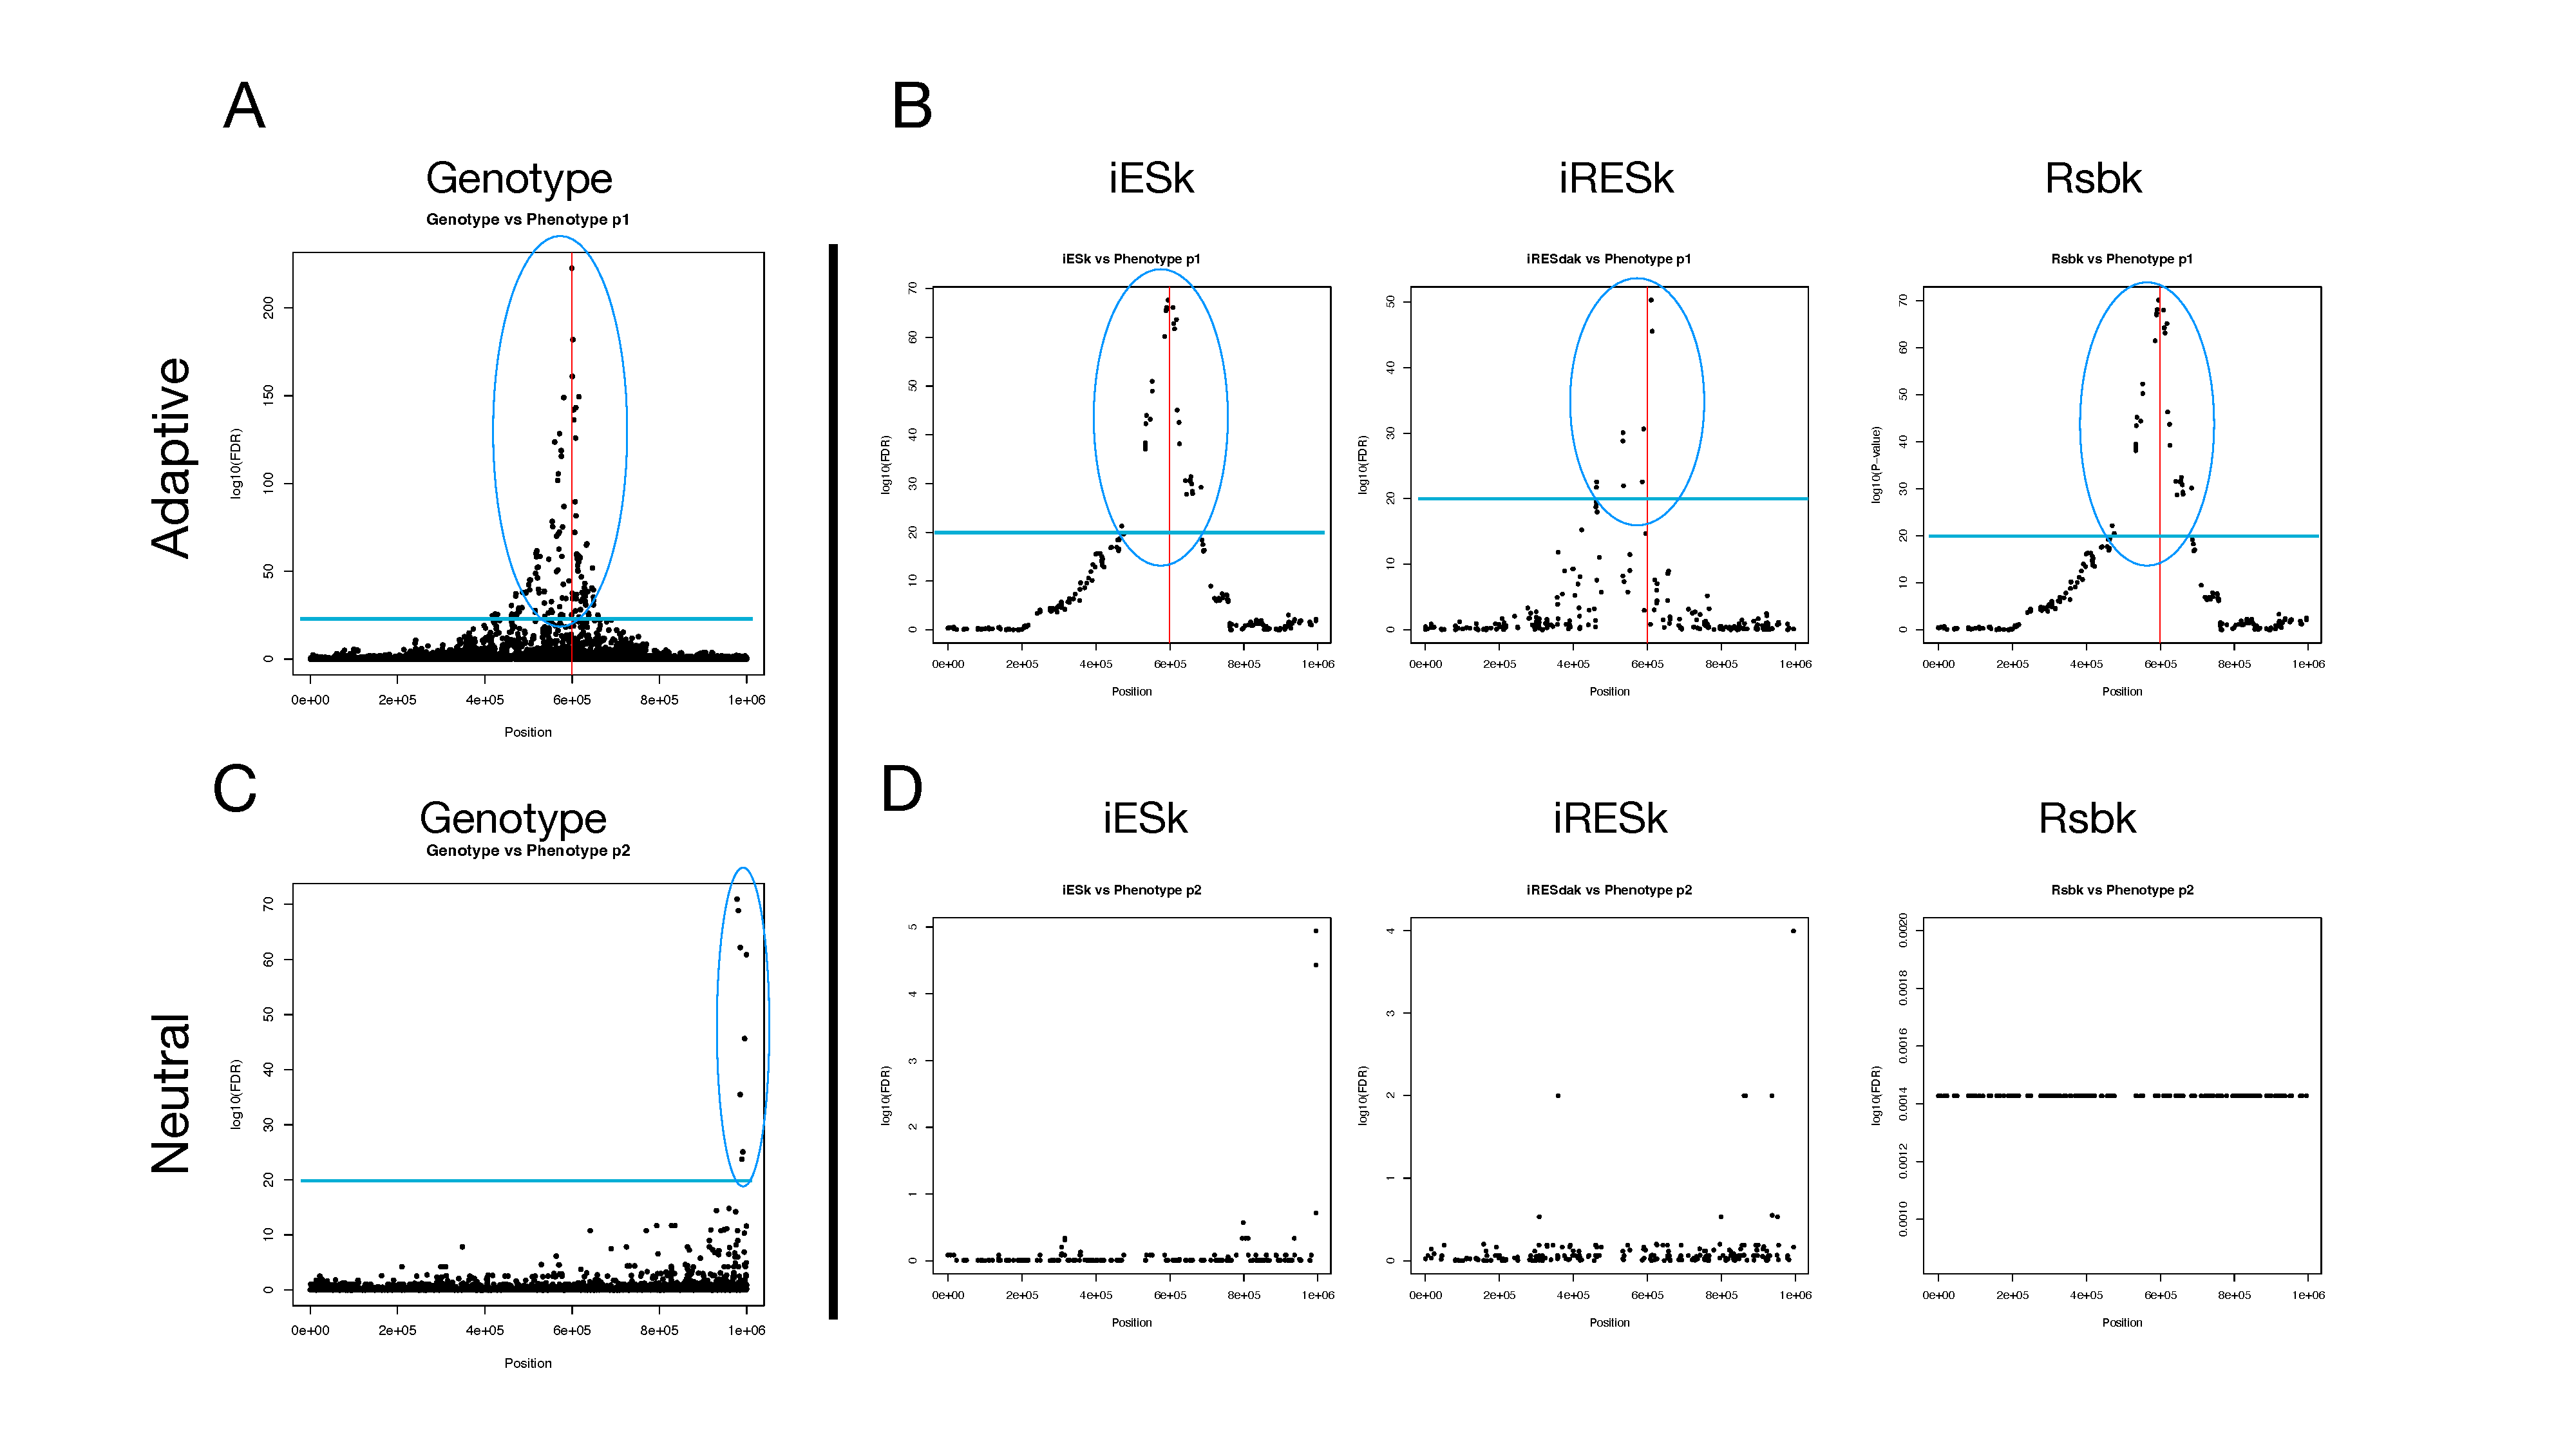
\includegraphics[scale=0.2]{./Example_EHHstatsGWAS.pdf}}
\caption{GWA analysis for genotype (A, C) and for EHH statistics (B, D). Two phenotypes are analyzed, one with adaptive effect (A, B) and one with neutral effect (C, D). The horizontal blue line and the blue circle sorrounding points indicate the positions with significant associations. Red line indicate the regions with mutations having additive effect on fitness at frequency higher than 0.05.}
\label{Example_EHHstatsGWAS}
\hspace*{-0.5cm}
\end{figure}

\subsection{Real Data Analysis}

\section{Discussion}

We provide a methodology to discriminate in one step the phenotypes that are affected by adaptive processes versus neutral. 
Advantages and disadvantages. Nevertheless, when the strength of the adaptive process affects regions that are also linked to regions affecting non-adaptive phenotypes, then the signal will be also observed, which may confound the interpretation of the results.
Statistical power of each statistic. 
Code to run
Develop an R function?

\bibliographystyle{genetics}
\bibliography{EHHGWAS}

%\newpage
%\beginsupplement
%
%\begin{figure}[h]
%{\includegraphics[scale=0.75]{./GammBiv_EW_plot_Fig1.pdf}}
%\caption{Comparison of distributions between Eyre-Walker (EW) function and a Gamma Bivariant correlated distribution. The selective effect follows a gamma distribution with shape=0.2 and mean=$-0.03$ for negative side and shape=1 and mean=0.01 for positive side and a proportion of positive variants of 5e-3. the first row show the distribution of Selective (x-axis) and Phenotype (y-axis) effects for three different conditions given the EW function (left: $\tau=0.0$, $sd=0.5$, center: $\tau=0.25$, $sd=0.4$, right: $\tau=0.50$, $sd=0.4$), The second row show the distribution of Selective and Phenotype effects for three different correlation conditions (left: $\rho=0.0$, center: $\rho=0.80$ and  left $\rho=0.95$) using the Gamma distribution. }
%\label{comEWvsBiv}
%\hspace*{-0.5cm}
%\end{figure}
%
%\begin{figure}[h]
%{\includegraphics[scale=0.45]{./Dist_ALLScenarios1.pdf}}
%\caption{Distribution of the beneficial and deleterious mutations for scenarios 1,2,3, and 4. Each row indicates one scenario. Horizontal lines indicate the optimal phenotypic value for the first (black) and second scenario (blue). Vertical line separate deleterious from beneficial selective effects. At left side, Black circles indicate the mutations for the initial environment, at central, purple dots indicate the displacement of selective effects for standing mutations at the new second environment.  At right side, the distribution of new mutations at the second environment (in blue) in relation to its selective and phenotype effect.}
%\label{DistALLScenarios1}
%\hspace*{-0.5cm}
%\end{figure}
%
%\begin{figure}[h]
%{\includegraphics[scale=0.45]{./Dist_ALLScenarios2.pdf}}
%\caption{Distribution of the beneficial and deleterious mutations for scenarios 5,6,7, and 8. Each row indicates one scenario. Horizontal lines indicate the optimal phenotypic value for the first (black) and second scenario (blue). Vertical line separate deleterious from beneficial selective effects. At left side, Black circles indicate the mutations for the initial environment, at central, purple dots indicate the displacement of selective effects for standing mutations at the new second environment.  At right side, the distribution of new mutations at the second environment (in blue) in relation to its selective and phenotype effect}
%\label{DistALLScenarios2}
%\hspace*{-0.5cm}
%\end{figure}
%
%\begin{figure}[h]
%{\includegraphics[scale=0.45]{./Dist_ALLScenarios3.pdf}}
%\caption{Distribution of the beneficial and deleterious mutations for scenarios 9 and 10. Each row indicates one scenario. Horizontal lines indicate the optimal phenotypic value for the first (black) and second scenario (blue). Vertical line separate deleterious from beneficial selective effects. At left side, Black circles indicate the mutations for the initial environment, at central, purple dots indicate the displacement of selective effects for standing mutations at the new second environment.  At right side, the distribution of new mutations at the second environment (in blue) in relation to its selective and phenotype effect}
%\label{DistALLScenarios3}
%\hspace*{-0.5cm}
%\end{figure}

\end{document}
